% Options for packages loaded elsewhere
\PassOptionsToPackage{unicode}{hyperref}
\PassOptionsToPackage{hyphens}{url}
%
\documentclass[
  man]{apa7}
\usepackage{amsmath,amssymb}
\usepackage{lmodern}
\usepackage{iftex}
\ifPDFTeX
  \usepackage[T1]{fontenc}
  \usepackage[utf8]{inputenc}
  \usepackage{textcomp} % provide euro and other symbols
\else % if luatex or xetex
  \usepackage{unicode-math}
  \defaultfontfeatures{Scale=MatchLowercase}
  \defaultfontfeatures[\rmfamily]{Ligatures=TeX,Scale=1}
\fi
% Use upquote if available, for straight quotes in verbatim environments
\IfFileExists{upquote.sty}{\usepackage{upquote}}{}
\IfFileExists{microtype.sty}{% use microtype if available
  \usepackage[]{microtype}
  \UseMicrotypeSet[protrusion]{basicmath} % disable protrusion for tt fonts
}{}
\makeatletter
\@ifundefined{KOMAClassName}{% if non-KOMA class
  \IfFileExists{parskip.sty}{%
    \usepackage{parskip}
  }{% else
    \setlength{\parindent}{0pt}
    \setlength{\parskip}{6pt plus 2pt minus 1pt}}
}{% if KOMA class
  \KOMAoptions{parskip=half}}
\makeatother
\usepackage{xcolor}
\usepackage{graphicx}
\makeatletter
\def\maxwidth{\ifdim\Gin@nat@width>\linewidth\linewidth\else\Gin@nat@width\fi}
\def\maxheight{\ifdim\Gin@nat@height>\textheight\textheight\else\Gin@nat@height\fi}
\makeatother
% Scale images if necessary, so that they will not overflow the page
% margins by default, and it is still possible to overwrite the defaults
% using explicit options in \includegraphics[width, height, ...]{}
\setkeys{Gin}{width=\maxwidth,height=\maxheight,keepaspectratio}
% Set default figure placement to htbp
\makeatletter
\def\fps@figure{htbp}
\makeatother
\setlength{\emergencystretch}{3em} % prevent overfull lines
\providecommand{\tightlist}{%
  \setlength{\itemsep}{0pt}\setlength{\parskip}{0pt}}
\setcounter{secnumdepth}{-\maxdimen} % remove section numbering
% Make \paragraph and \subparagraph free-standing
\ifx\paragraph\undefined\else
  \let\oldparagraph\paragraph
  \renewcommand{\paragraph}[1]{\oldparagraph{#1}\mbox{}}
\fi
\ifx\subparagraph\undefined\else
  \let\oldsubparagraph\subparagraph
  \renewcommand{\subparagraph}[1]{\oldsubparagraph{#1}\mbox{}}
\fi
\newlength{\cslhangindent}
\setlength{\cslhangindent}{1.5em}
\newlength{\csllabelwidth}
\setlength{\csllabelwidth}{3em}
\newlength{\cslentryspacingunit} % times entry-spacing
\setlength{\cslentryspacingunit}{\parskip}
\newenvironment{CSLReferences}[2] % #1 hanging-ident, #2 entry spacing
 {% don't indent paragraphs
  \setlength{\parindent}{0pt}
  % turn on hanging indent if param 1 is 1
  \ifodd #1
  \let\oldpar\par
  \def\par{\hangindent=\cslhangindent\oldpar}
  \fi
  % set entry spacing
  \setlength{\parskip}{#2\cslentryspacingunit}
 }%
 {}
\usepackage{calc}
\newcommand{\CSLBlock}[1]{#1\hfill\break}
\newcommand{\CSLLeftMargin}[1]{\parbox[t]{\csllabelwidth}{#1}}
\newcommand{\CSLRightInline}[1]{\parbox[t]{\linewidth - \csllabelwidth}{#1}\break}
\newcommand{\CSLIndent}[1]{\hspace{\cslhangindent}#1}
\ifLuaTeX
\usepackage[bidi=basic]{babel}
\else
\usepackage[bidi=default]{babel}
\fi
\babelprovide[main,import]{english}
% get rid of language-specific shorthands (see #6817):
\let\LanguageShortHands\languageshorthands
\def\languageshorthands#1{}
% Manuscript styling
\usepackage{upgreek}
\captionsetup{font=singlespacing,justification=justified}

% Table formatting
\usepackage{longtable}
\usepackage{lscape}
% \usepackage[counterclockwise]{rotating}   % Landscape page setup for large tables
\usepackage{multirow}		% Table styling
\usepackage{tabularx}		% Control Column width
\usepackage[flushleft]{threeparttable}	% Allows for three part tables with a specified notes section
\usepackage{threeparttablex}            % Lets threeparttable work with longtable

% Create new environments so endfloat can handle them
% \newenvironment{ltable}
%   {\begin{landscape}\centering\begin{threeparttable}}
%   {\end{threeparttable}\end{landscape}}
\newenvironment{lltable}{\begin{landscape}\centering\begin{ThreePartTable}}{\end{ThreePartTable}\end{landscape}}

% Enables adjusting longtable caption width to table width
% Solution found at http://golatex.de/longtable-mit-caption-so-breit-wie-die-tabelle-t15767.html
\makeatletter
\newcommand\LastLTentrywidth{1em}
\newlength\longtablewidth
\setlength{\longtablewidth}{1in}
\newcommand{\getlongtablewidth}{\begingroup \ifcsname LT@\roman{LT@tables}\endcsname \global\longtablewidth=0pt \renewcommand{\LT@entry}[2]{\global\advance\longtablewidth by ##2\relax\gdef\LastLTentrywidth{##2}}\@nameuse{LT@\roman{LT@tables}} \fi \endgroup}

% \setlength{\parindent}{0.5in}
% \setlength{\parskip}{0pt plus 0pt minus 0pt}

% Overwrite redefinition of paragraph and subparagraph by the default LaTeX template
% See https://github.com/crsh/papaja/issues/292
\makeatletter
\renewcommand{\paragraph}{\@startsection{paragraph}{4}{\parindent}%
  {0\baselineskip \@plus 0.2ex \@minus 0.2ex}%
  {-1em}%
  {\normalfont\normalsize\bfseries\itshape\typesectitle}}

\renewcommand{\subparagraph}[1]{\@startsection{subparagraph}{5}{1em}%
  {0\baselineskip \@plus 0.2ex \@minus 0.2ex}%
  {-\z@\relax}%
  {\normalfont\normalsize\itshape\hspace{\parindent}{#1}\textit{\addperi}}{\relax}}
\makeatother

\makeatletter
\usepackage{etoolbox}
\patchcmd{\maketitle}
  {\section{\normalfont\normalsize\abstractname}}
  {\section*{\normalfont\normalsize\abstractname}}
  {}{\typeout{Failed to patch abstract.}}
\patchcmd{\maketitle}
  {\section{\protect\normalfont{\@title}}}
  {\section*{\protect\normalfont{\@title}}}
  {}{\typeout{Failed to patch title.}}
\makeatother

\usepackage{xpatch}
\makeatletter
\xapptocmd\appendix
  {\xapptocmd\section
    {\addcontentsline{toc}{section}{\appendixname\ifoneappendix\else~\theappendix\fi\\: #1}}
    {}{\InnerPatchFailed}%
  }
{}{\PatchFailed}
\keywords{big team, science, authorship, credit\newline\indent Word count: X}
\DeclareDelayedFloatFlavor{ThreePartTable}{table}
\DeclareDelayedFloatFlavor{lltable}{table}
\DeclareDelayedFloatFlavor*{longtable}{table}
\makeatletter
\renewcommand{\efloat@iwrite}[1]{\immediate\expandafter\protected@write\csname efloat@post#1\endcsname{}}
\makeatother
\usepackage{lineno}

\linenumbers
\usepackage{csquotes}
\makeatletter
\renewcommand{\paragraph}{\@startsection{paragraph}{4}{\parindent}%
  {0\baselineskip \@plus 0.2ex \@minus 0.2ex}%
  {-1em}%
  {\normalfont\normalsize\bfseries\typesectitle}}

\renewcommand{\subparagraph}[1]{\@startsection{subparagraph}{5}{1em}%
  {0\baselineskip \@plus 0.2ex \@minus 0.2ex}%
  {-\z@\relax}%
  {\normalfont\normalsize\bfseries\itshape\hspace{\parindent}{#1}\textit{\addperi}}{\relax}}
\makeatother

\ifLuaTeX
  \usepackage{selnolig}  % disable illegal ligatures
\fi
\IfFileExists{bookmark.sty}{\usepackage{bookmark}}{\usepackage{hyperref}}
\IfFileExists{xurl.sty}{\usepackage{xurl}}{} % add URL line breaks if available
\urlstyle{same} % disable monospaced font for URLs
\hypersetup{
  pdftitle={Who does big team science?},
  pdfauthor={Erin M. Buchanan1 \& Savannah C. Lewis2},
  pdflang={en-EN},
  pdfkeywords={big team, science, authorship, credit},
  hidelinks,
  pdfcreator={LaTeX via pandoc}}

\title{Who does big team science?}
\author{Erin M. Buchanan\textsuperscript{1} \& Savannah C. Lewis\textsuperscript{2}}
\date{}


\shorttitle{Big Team Science}

\authornote{

Erin M. Buchanan is a Professor of Cognitive Analytics at Harrisburg University of Science and Technology. Savannah C. Lewis is a graduate student at the University of Alabama.

Thank you to Dwayne Lieck for providing an extensive list of large scale projects for this manuscript.

The authors made the following contributions. Erin M. Buchanan: Conceptualization, Data curation, Formal Analysis, Methodology, Project administration, Visualization, Writing -- original draft, Writing -- review \& editing; Savannah C. Lewis: Conceptualization, Data curation, Methodology, Project administration, Writing -- original draft, Writing -- review \& editing.

Correspondence concerning this article should be addressed to Erin M. Buchanan, 326 Market St., Harrisburg, PA 17101. E-mail: \href{mailto:ebuchanan@harrisburgu.edu}{\nolinkurl{ebuchanan@harrisburgu.edu}}

}

\affiliation{\vspace{0.5cm}\textsuperscript{1} Harrisburg University of Science and Technology\\\textsuperscript{2} University of Alabama}

\abstract{%
This paper will examine the nature of publications in Big Team Science (BTS) - large-scale collaborations between multiple researchers at multiple institutions. As interest in BTS increases, it is useful to explore who is currently involved in BTS projects to determine diversity in both research subject and researcher representation. The types of publication outlets, number of publications, and subject areas of publication will be presented to summarize the publications in BTS. Information about authors included in BTS will be presented including career length, numbers of publications/impact variables, education, and affiliation. Last, we will explore the representation of geopolitical regions by examining affiliation location to explore the impact of BTS on the de-WEIRD movement to diversify researcher representation.
}



\begin{document}
\maketitle

According to the Oxford English dictionary, collaboration is two or more
people working together to achieve a certain goal (OED, 2016).
Collaboration in scientific endeavors involves multiple researchers at
(potentially) multiple institutions to communicate and work together to
advance knowledge in their chosen field. Collaboration can manifest
uniquely in each project dependent on the skill sets, hypotheses, and
perspectives of collaborators. While collaboration is not new in
science, the current interest of ``big team science'' is increasing
(Coles et al., 2022; Forscher et al., 2020; N. Stewart et al., 2017). Big team science projects
and/or organizations utilize and run on large-scale collaboration to
ensure that diverse populations and ideas are brought into research
projects, which in turn allows for more reliability and generalizability
in the results and method of the study. For this study, Big Team Science
(BTS) will be defined as a collaboration of ten or more authors from at
least ten different institutions.

BTS appears to be increasing as a result of two sources: 1) increasing
globalization and technology that allows for real-time interdisciplinary
research, and 2) increasing interest in reproducibility, replication,
and generalizability (Maxwell et al., 2015; Nelson et al., 2018; Zwaan et al., 2018).
Technological advances have provided easier ways to collaborate with
people who are from other universities and countries through document
sharing platforms (e.g., Google, GitHub, and the Open Science
Framework), video chatting platforms (e.g., Zoom, Microsoft Teams), and
messaging and project management platforms (e.g., Slack, Trello,
when2meet, etc.). The credibility movement seems to suggest that by
having both collaborations that span across the globe and subfield of
psychology, age groups, and education levels should help to drive
psychological science in the path of better materials, reliability,
generalizability and more robust sample size in a study
(Auspurg \& Brüderl, 2021; LeBel et al., 2018; Nosek \& Lakens, 2014b).

The credibility movement was originally defined by a focus on large
scale replications using in collaborative environments (Vazire et al., 2022).
Generally, the movement has been driven by early career researchers
(i.e., those who are within five years of their first appointment)
(Maizey \& Tzavella, 2019); however, there are no large meta-scientific
investigations on this specific topic to date. Potentially, the lack of
investigation is tied to the newness of the large-scale research in many
fields, as it is only in recent years that publications like the Open
Science Collaboration (Open Science Collaboration, 2015), Many Labs
Collaborations (Buttrick et al., 2020; Ebersole et al., 2020, 2016; Klein et al., 2022; for example, Klein et al., 2018; Mathur et al., 2020; Skorb et al., 2020) or the first papers
from the Psychological Science Accelerator (Bago et al., 2022; Dorison et al., 2022; Jones et al., 2021; Legate et al., 2022; Moshontz et al., 2018; Wang et al., 2021). Generally, the
researcher incentive for replication was low: journals often prioritize
``novel'' or new results which led to rejection of replication manuscripts
and publication bias (Franco et al., 2014; Hubbard \& Armstrong, 1997; Nosek et al., 2012), the
``failure'' to replicate was often placed on the replication team as ``bad
science'' rather than a careful consideration of publication biases and
(potential) questionable research practices (Ioannidis, 2015; Klein et al., 2022; Maxwell et al., 2015), and why should someone want to spend time and
resources on an answer we already ``know'' (Isager et al., 2021a, 2021b)?

However, the success and interest in the large-scale reproducibility
projects (Errington et al., 2021; Open Science Collaboration, 2015), paired
with the meta-scientific publications focusing on researcher practices
and incentive structures (John et al., 2012; Silberzahn et al., 2018) led to a
change in journal guidelines and incentives for researchers interested
in participating in large-scale replication studies (Grahe, 2014; Kidwell et al., 2016; Mayo-Wilson et al., 2021; Nosek et al., 2015). For example, the support
for Registered Reports, papers accepted before the data has been
collected (Nosek \& Lakens, 2014a; S. Stewart et al., 2020), and entire sub-sections of
journals devoted to only replication studies (e.g., \emph{Nature, Royal
Society Open Science, Advances in Methods and Practices in Psychological
Science}) has allowed researchers to invest in projects that they know
should be published when the project is complete. Further, the
implementation of the Transparency and Openness Guidelines (Nosek et al., 2015)
and the Contributor Role Taxonomy (CRediT) system (Allen et al., 2019) have
pushed journals and researchers to promote more open, inclusive
publication practices.

The credibility movement has been mirrored by the calls for
diversification or de-WEIRDing (e.g., Western, Educated, Industrialized,
Rich, and Democratic) scientific research (Henrich et al., 2010; Newson et al., 2021; Rad et al., 2018) by improving representation in research samples. Like the
large-scale studies in Physics ({``A Philosophical Case for Big Physics,''} 2021; Castelnovo et al., 2018) and
Biology (Collins et al., 2003), the social sciences struggle to represent the
breadth of humanity across both researcher and population
characteristics. Now, grassroots organizations, such as the
Psychological Science Accelerator (Moshontz et al., 2018), ManyBabies
(\url{https://manybabies.github.io/}), NutNet (\url{https://nutnet.org/}), and
DRAGNet (\url{https://dragnetglobal.weebly.com/}) can begin to tackle these
issues by recruiting research labs from all over the globe to provide
diversity in geographic, linguistic, and researcher representation.
Publications have examined the global understanding of morality, face
processing, COVID-19 information signaling, and more (Bago et al., 2022; Dorison et al., 2022; Jones et al., 2021; Legate et al., 2022; Van Bavel et al., 2022; Wang et al., 2021). While
these organizations and one-time groups for BTS studies have provided an
incredible wealth of data for the scientific community, we do not yet
know exactly \emph{who} is involved with, and benefits from, the BTS and
credibility movement. Publications on BTS generally explore challenges,
lessons learned, and the need for BTS (Coles et al., 2022; Forscher et al., 2020).

Therefore, the goal of this manuscript is to examine the \emph{people}
involved in BTS projects. We specifically expect to examine ICSR's
Research Themes of inclusivity, research careers, and research
globalization. As we examine these themes, it will bring new knowledge
of how BTS projects impact each theme and field of study. We see an
increase in interest and publications in BTS but we do not yet know if
this uptick in large-scale projects has diversified the \emph{people}
involved in BTS. While a few publications have noted that BTS appears to
be early career researchers (Maizey \& Tzavella, 2019), no one has systematically
investigated this perception. Further, it is unclear if the focus of
de-WEIRDing science has only focused on the representation of the
research participants or if it has also improved the representation of
researchers outside of North America and Europe. Last, who runs these
BTS projects? Do we see an increase in diversity for the authors who
generally receive the most credit for these projects (i.e., first
several author(s) and last author)? As hiring and promoting practices
often place a heavy weight on publications and especially ``influential''
publications, it becomes necessary to critically examine the
representation present in authorship in BTS projects.

\hypertarget{potential-outlets}{%
\section{Potential Outlets}\label{potential-outlets}}

We will aim for high impact broad scope journals such as \emph{Science},
\emph{Nature} or \emph{Nature Human Behaviour}. Other journals would include
review publications within psychology to compare the social sciences to
other sciences: \emph{Perspectives in Psychological Science}, \emph{Psychological
Bulletin}, \emph{Psychological Review}, or \emph{Current Directions in
Psychological Science}.

\hypertarget{research-questions}{%
\section{Research Questions}\label{research-questions}}

\begin{itemize}
\tightlist
\item
  Research Question 1: What publication sources publish big team
  science papers?
\item
  Research Question 2: What are the types of articles that are being
  published in big team science?
\item
  Research Question 3: Who is involved in big team science?
\end{itemize}

For each of these research questions, we will examine the overall
results of all big team research projects, and examine for change in
result trends across years of publication. Below we detail our methods
and the ICSR/Scopus data to answer these questions, along with examples
of the statistical results we expect to report in the manuscript. We
began this project with data using Google Scholar and ORCID information.
These sources were severely limited in their scope and breadth, as they
are often curated with automatic processes or self-entered data, and we
believe that access to Scopus and ICSR would allow us to accurately
portray the BTS movement and its impact on diversity across many fields.
The novelty of this project is that it would focus on all of published
works, rather than a specific subfield (like Psychology) and give a lens
into global representation in science that would otherwise not be
achieved with open-source databases.

\hypertarget{method}{%
\section{Method}\label{method}}

\hypertarget{publications}{%
\subsection{Publications}\label{publications}}

We have defined \textbf{BTS publications} as publications with at least 10
authors at 10 different institutions that were published in
peer-reviewed journals or had posted a full paper pre-print. We will use
data from 1970 and forward in the publications (\texttt{ani}) database, as it
is noted online that this time period includes cited references for
calculation of several of our variables described below. We will analyze
our results based on the big four subject areas: Physical Sciences,
Health Sciences, Social Sciences, and Life Sciences. We filtered the
database to include articles, articles in press, business articles,
conference papers, data papers, preprints, and surveys using Elsevier's
classification system.

\hypertarget{data-curation}{%
\subsection{Data Curation}\label{data-curation}}

\hypertarget{rq1-publisher-information.}{%
\subsubsection{RQ1: Publisher Information.}\label{rq1-publisher-information.}}

Using these criteria, we will extract the following information for
publication sources: the name of the publication (source title), subject
area (both the large four subject areas and the smaller four digit all
science journal classification ASJC codes). We will examine journal
impact using the Source Normalized Impact per Paper from the journal
(\texttt{sources}) database.

\hypertarget{rq2-publication-information.}{%
\subsubsection{RQ2: Publication Information.}\label{rq2-publication-information.}}

For each publication of the identified BTS publications, we will analyze
the full four digit ASJC subject areas codes for each of the larger four
subject areas and the keywords present for these publications.

\hypertarget{rq3-author-information.}{%
\subsubsection{RQ3: Author Information.}\label{rq3-author-information.}}

The author list will then be extracted from each publication. Next, we
will use the author (\texttt{au}) and affiliation (\texttt{af}) array to curate a list
of all publications and author information included in BTS papers. We
will use these two arrays with the publication array to calculate the
variables described below.

\textbf{\emph{Career Length}}. Career length for each author will be defined as
the year of the first publication listed for each author.

\textbf{\emph{Institution and Geopolitical Region}} . We will use the affiliation
ids and country to gather information about the places of education
and/or employment for authors. Country will likely be binned into United Nation Region, Sub-Region, or smaller clusters for analyses.

\textbf{\emph{Education}}. We will also collect degree information from the author table.

\textbf{\emph{Types of Publications}}. We will gather information from the
publication type variable for each author publication to present
information about the types of papers BTS authors publish.

\textbf{\emph{Publication Metrics}}. For each author, we will calculate the total
number of publications, and the h-index. The h-index represents the
highest \emph{h} number of publications that have at least \emph{h} citations.

\hypertarget{data-analysis}{%
\subsection{Data analysis}\label{data-analysis}}

\hypertarget{rq1-publisher-information.-1}{%
\subsubsection{RQ1: Publisher Information.}\label{rq1-publisher-information.-1}}

To present results on this research question, we will analyze:

\begin{itemize}
\tightlist
\item
  Number of articles for inclusion: total, separated by four subject
  areas, presenting graphics of the number of publication across time
  total
\end{itemize}

\emph{Number of articles}. The total number of articles included in this analysis was 510334 including 445301 Health Sciences articles, 228194
Physical Sciences articles, 26652 Social Sciences articles, and
307514 Life Sciences articles. Articles could be classified into
multiple categories. Figure X shows the number of articles published across time for each of the four large subject areas.

\begin{figure}
\centering
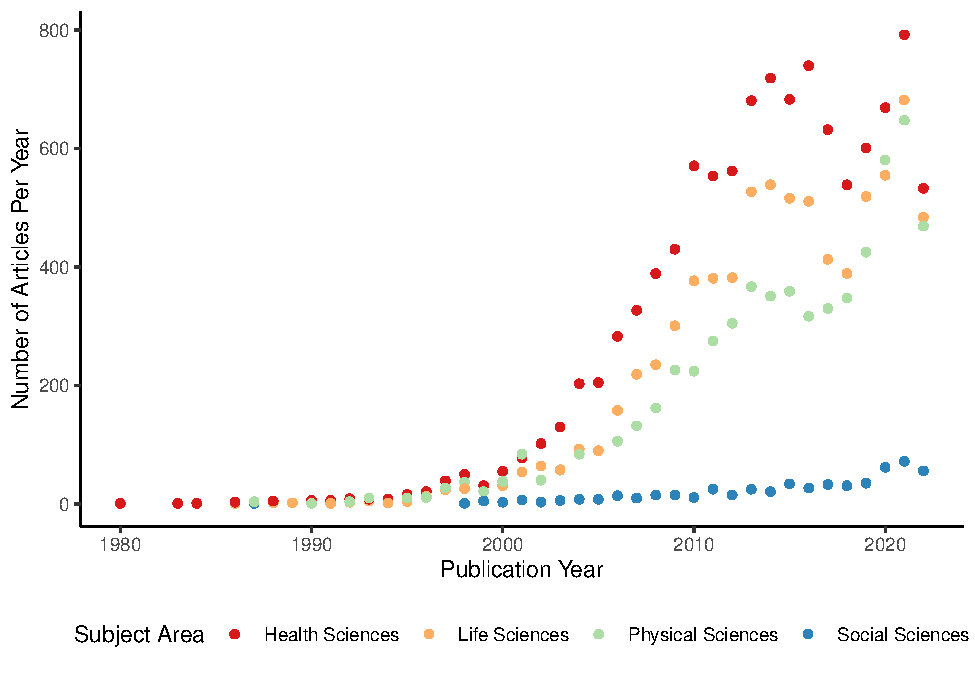
\includegraphics{manuscript_scopus_files/figure-latex/fig-pub-time-1.pdf}
\caption{\label{fig:fig-pub-time}Number of big-team science publications separated by four large subject areas across years.}
\end{figure}

\begin{itemize}
\tightlist
\item
  Number of distinct journals within each of the four subject areas
\end{itemize}

\emph{Number of journals}. The number of distinct journals big team science articles were published
in was 14924 with 6559 journals in Health Sciences,
5787 journals in Physical Sciences, 2500
journals in Social Sciences, and 4187 journals in Life
Sciences. The descriptive statistics for the Source Normalized Impact
per Paper is presented in Table X. For comparison, the SNIP descriptive
statistics for all papers is shown in Table X.

\begin{table}[tbp]

\begin{center}
\begin{threeparttable}

\caption{\label{tab:tab-snip}Big-Team Science SNIP Values}

\begin{tabular}{llllll}
\toprule
Subject Area & \multicolumn{1}{c}{M} & \multicolumn{1}{c}{SD} & \multicolumn{1}{c}{Minimum} & \multicolumn{1}{c}{Median} & \multicolumn{1}{c}{Maximum}\\
\midrule
Health Sciences & 2.36 & 3.59 & 0.00 & 1.58 & 173.93\\
Physical Sciences & 1.57 & 1.17 & 0.00 & 1.27 & 30.40\\
Social Sciences & 1.94 & 1.72 & 0.00 & 1.52 & 30.40\\
Life Sciences & 2.02 & 1.60 & 0.00 & 1.51 & 19.07\\
\bottomrule
\end{tabular}

\end{threeparttable}
\end{center}

\end{table}

\begin{table}[tbp]

\begin{center}
\begin{threeparttable}

\caption{\label{tab:tab-snip-all}All Journal Articles SNIP Values}

\begin{tabular}{llllll}
\toprule
Subject Area & \multicolumn{1}{c}{M} & \multicolumn{1}{c}{SD} & \multicolumn{1}{c}{Minimum} & \multicolumn{1}{c}{Median} & \multicolumn{1}{c}{Maximum}\\
\midrule
Health Sciences & 1.45 & 2.87 & 0.00 & 1.15 & 173.93\\
Physical Sciences & 1.08 & 0.77 & 0.00 & 0.97 & 30.40\\
Social Sciences & 1.32 & 1.03 & 0.00 & 1.15 & 30.40\\
Life Sciences & 1.19 & 0.86 & 0.00 & 1.06 & 19.07\\
\bottomrule
\end{tabular}

\end{threeparttable}
\end{center}

\end{table}

\hypertarget{rq2-publication-information.-1}{%
\subsubsection{RQ2: Publication Information.}\label{rq2-publication-information.-1}}

For each publication, we will examine:

\begin{itemize}
\tightlist
\item
  The totals of the number of articles published within the smaller
  subject area classifications. We will visualize these differences to show the areas of interest for each of the four large subject areas.
\end{itemize}

\begin{figure}
\centering
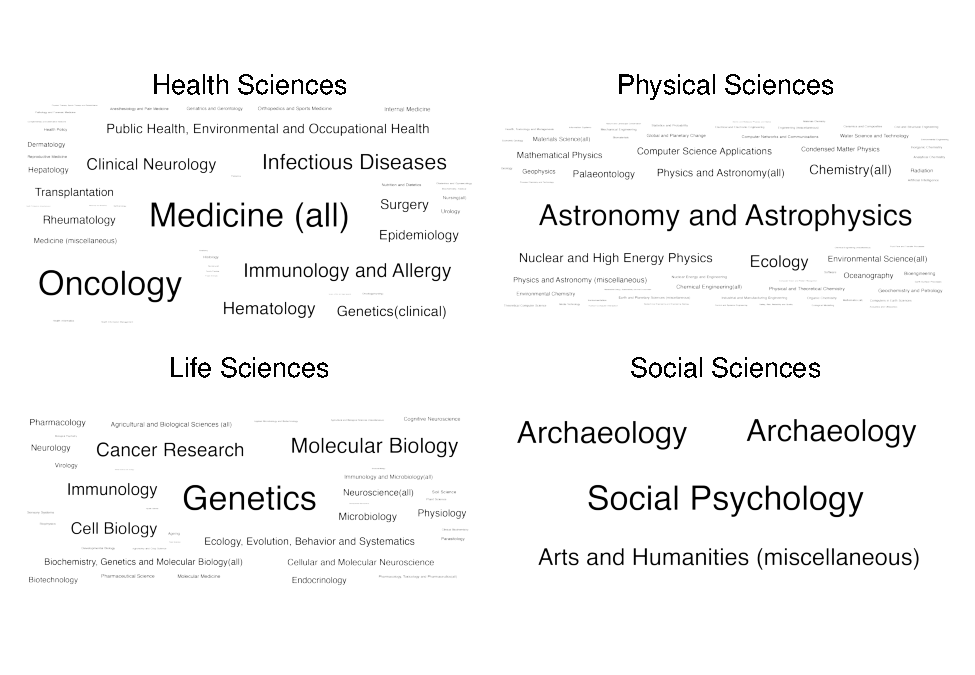
\includegraphics{manuscript_scopus_files/figure-latex/fig-clouds-1.pdf}
\caption{\label{fig:fig-clouds}Journal Areas for Big-Team Science Publications by Subject Area}
\end{figure}

\begin{itemize}
\tightlist
\item
  The keywords present in the publications data overall to identify
  trends and common themes in the publications for the four subject
  areas using visualizations (wordclouds) to depict the common
  keywords.
\end{itemize}

\begin{figure}
\centering
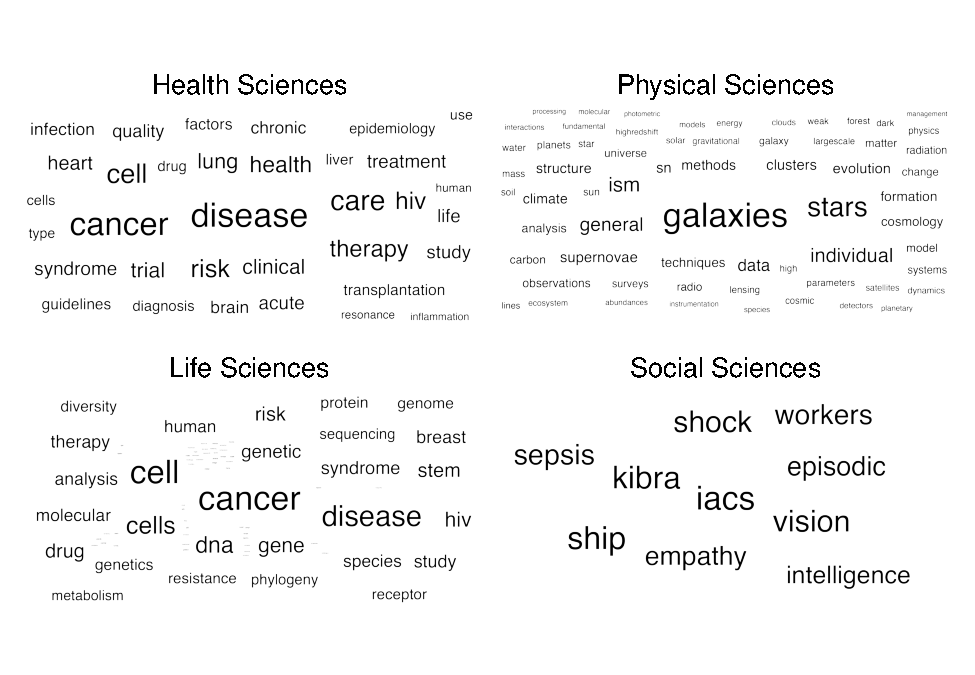
\includegraphics{manuscript_scopus_files/figure-latex/fig-keywords-1.pdf}
\caption{\label{fig:fig-keywords}Keyword Analysis for Each of the Four Subject Areas.}
\end{figure}

\hypertarget{rq3-authors.}{%
\subsubsection{RQ3: Authors.}\label{rq3-authors.}}

We will first present:

\begin{itemize}
\tightlist
\item
  The total number of unique authors
\end{itemize}

The total number of unique authors across all publications was
3047067.

\begin{itemize}
\tightlist
\item
  Statistics (mean, standard deviation, minimum, maximum, median) on
  the number of authors included on publications.
\end{itemize}

The mean number of authors per publication was \emph{M} = 49.90
(\emph{SD} = 207.01, \emph{Med} = 19) with a range of
10 to 5155.

\begin{itemize}
\tightlist
\item
  We will present visualizations of these results across time.
\end{itemize}

\begin{figure}
\centering
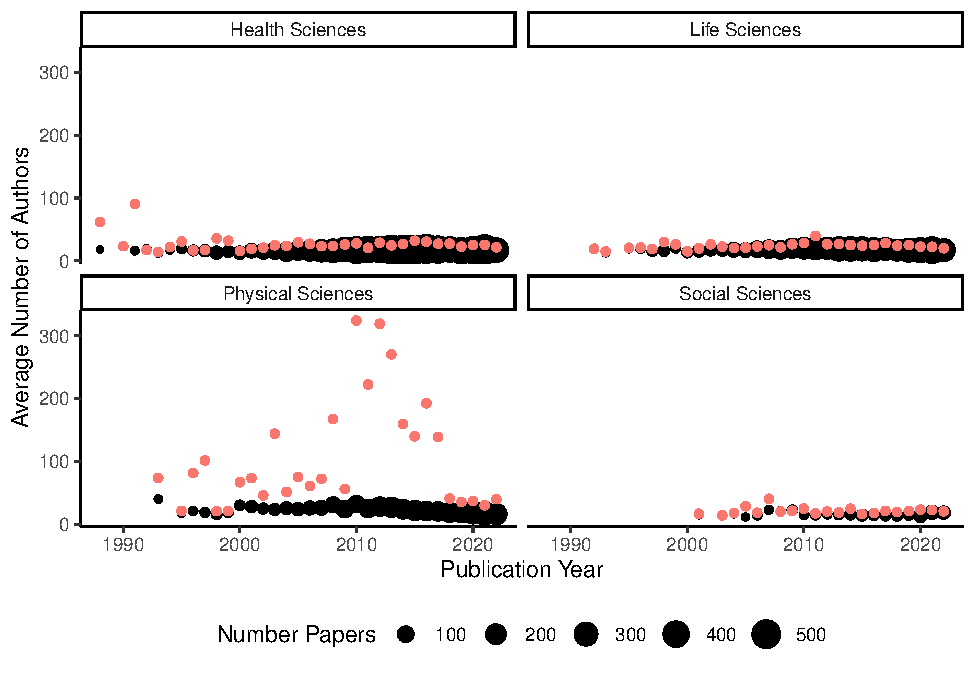
\includegraphics{manuscript_scopus_files/figure-latex/fig-author-year-1.pdf}
\caption{\label{fig:fig-author-year}Number of authors included on big-team science papers per year by subject area. Colored dots indicate the mean number of authors, while the black dots represent the median number of authors. The size of the black dots indicate the number of papers in that year.}
\end{figure}

We will use the 95\% confidence interval to make all claims of predictors
or effects different zero. The confidence interval that does not include
zero would be considered different from zero (to four decimal places).
We make no directional predictions.

\textbf{\emph{Career Length}}.

\begin{itemize}
\tightlist
\item
  We will create a visualization of the trend and variance of
  researcher career length across publication years.
\end{itemize}

\begin{figure}
\centering
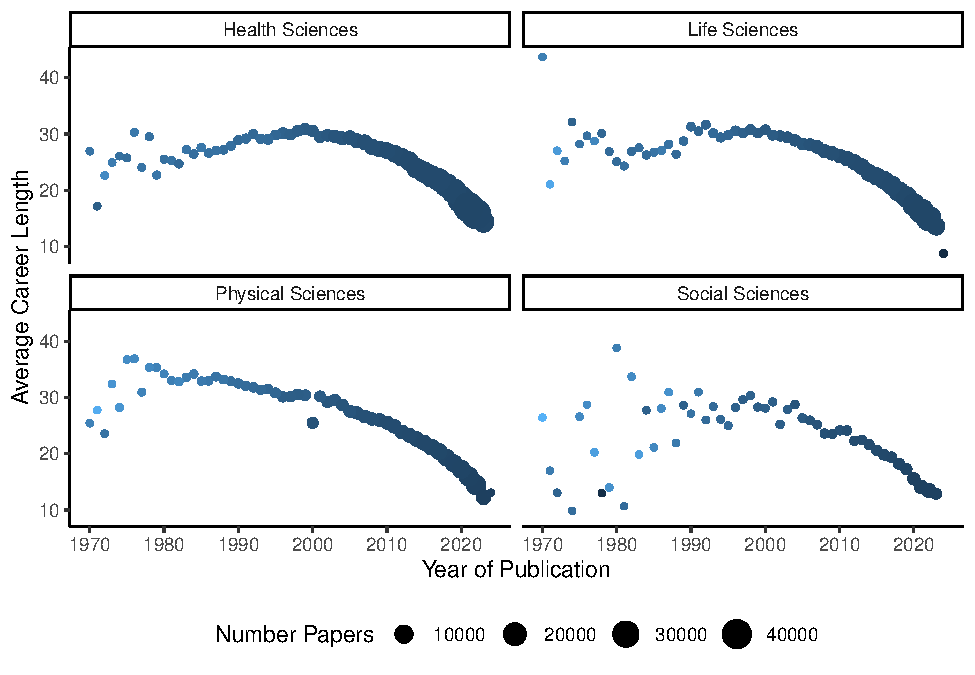
\includegraphics{manuscript_scopus_files/figure-latex/fig-career-1.pdf}
\caption{\label{fig:fig-career}Average career length for big-team science authors. Larger dots indicate more papers for each estimation. Lighter colored dots mean less variability in author career length, while darker dots mean more variability in career length.}
\end{figure}

\begin{itemize}
\tightlist
\item
  To analyze trends over time, we will calculate the average career
  length for each publication (i.e., average the author career length
  to create one score for each paper) and run a regression analysis
  using career length to predict year of publication. In order to show
  variance between individuals, we calculate the standard deviation of
  career length for each publication and run a regression analysis
  using this variance representation to predict publication year.
  These two variables will be used together.
\item
  Negative slopes would indicate more young scholars in later years
  (i.e., lower average career length as time increases). Positive
  slopes would indicate older scholars in later years (i.e., higher
  average career length as time increases).
\item
  Negative slopes imply that variability decreases over the years, so
  the average career length is more homogeneous. Positive slopes imply
  that variability increases over the years, so the average career
  length is varied across individuals (lots of different types of
  scholars).
\item
  These analyses will be completed separately for each of the four
  large subject areas.
\end{itemize}

\begin{figure}
\centering
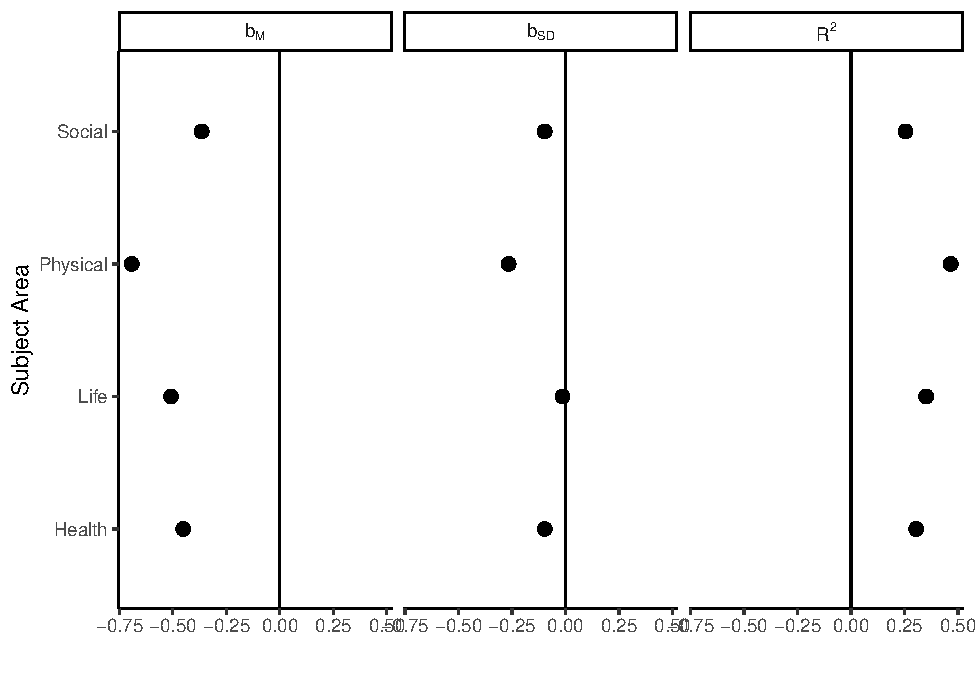
\includegraphics{manuscript_scopus_files/figure-latex/fig-career-results-1.pdf}
\caption{\label{fig:fig-career-results}Coefficient values for the average career length, variance in career length, and the effect size for each model predicting year of publication.}
\end{figure}

\textbf{\emph{Institution}}.

\begin{itemize}
\tightlist
\item
  We will summarize the number of affiliation ids present in BTS
  publications by subject area and visualize these results across
  time. These visualizations will be presented separately for each of
  the four subject areas.
\end{itemize}

The total number of unique affiliation across all papers was 463876.

\begin{figure}
\centering
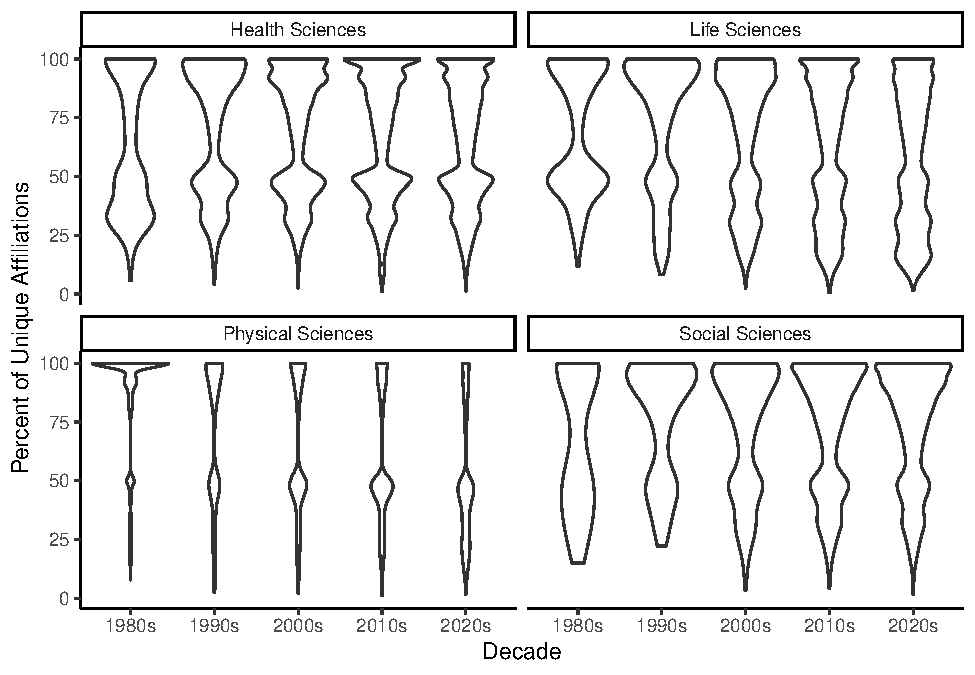
\includegraphics{manuscript_scopus_files/figure-latex/fig-inst-1.pdf}
\caption{\label{fig:fig-inst}Number of unique institutions involved in big-team science papers across decades.}
\end{figure}

\textbf{\emph{Types of Publications}}.

\begin{itemize}
\tightlist
\item
  We will summarize the coded types of publications for individuals.
\end{itemize}

\begin{figure}
\centering
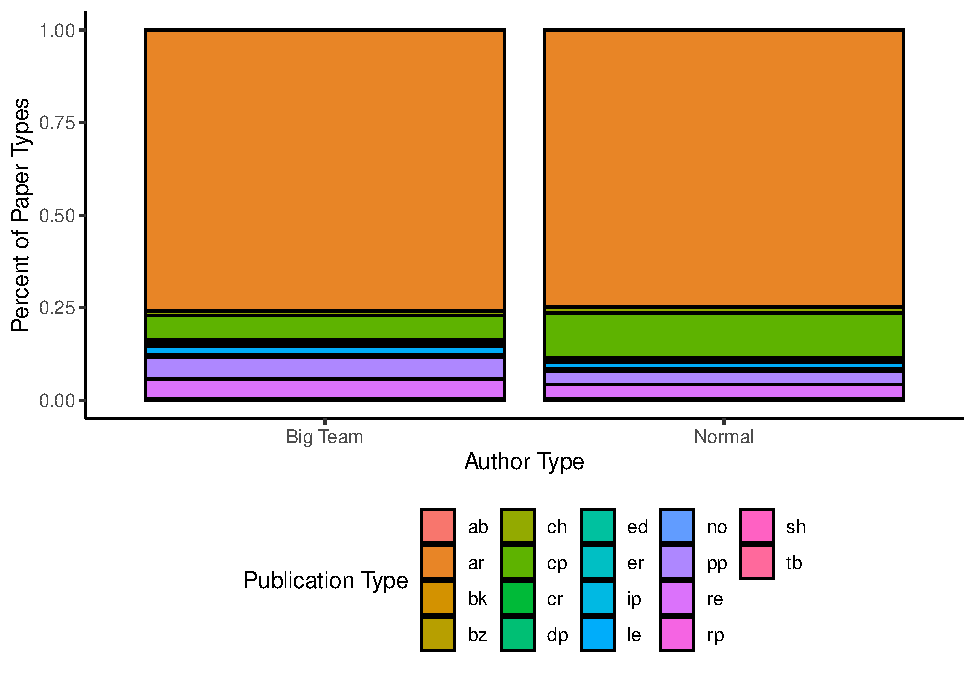
\includegraphics{manuscript_scopus_files/figure-latex/fig-pub-types-1.pdf}
\caption{\label{fig:fig-pub-types}Types of publications for big-team science and all authors.}
\end{figure}

\textbf{\emph{Publication Metrics}}.

\begin{itemize}
\tightlist
\item
  We will report descriptive statistics on the total number of
  publications and h-index for individuals overall.

  \begin{itemize}
  \tightlist
  \item
    Do this for each unique person and report averages
  \item
    Do this for each publication and create an average for each
    publication
  \end{itemize}
\end{itemize}

The average number of publications by authors on big team sciences
papers is \emph{M} = 38.37 (\emph{SD} =
102.54). The publication counts were averaged across
authors for each publication, and then these average publication counts
were averaged across publications \emph{M} = 162.50 (\emph{SD} =
155.17). The average variability (i.e., the average
standard deviation with authors of a manuscript) with publication counts
of a paper was \(M_{SD}\) = 164.27 (\(SD_{SD}\) =
127.21).

The same process was completed with \emph{h}-index for each author and
publication. The average \emph{h}-index for authors overall was \emph{M} =
33.65 (\emph{SD} = 127.34, \emph{Med} = 8.00). The
average \emph{h}-index for publications was \emph{M} = 198.87 (\emph{SD}
= 248.78), and the variability of \emph{h}-index across
manuscripts was \(M_{SD}\) = 211.80 (\(SD_{SD}\) =
238.53, \(Med_{Med}\) = 68.00).

\begin{itemize}
\tightlist
\item
  Next, we will use the same analyses described in the career length
  section to analyze trends over time. An increasing slope over time
  indicates that individuals who are publishing more are more
  represented in BTS over time (i.e., increasing numbers of scholars
  with higher publication rates), while a negative slope indicates
  more researchers with less publications.
\item
  A positive slope for standard deviation indicates increasing
  variance over time (i.e., more diversity in the individual
  publication rates), while a negative slope would indicate less
  diversity in researchers over time. While publication rates do not
  represent value as a researcher, they are often used in hiring and
  promotion decisions, and we will use this variable as a proxy to
  gauge the diversity in scholars represented in big teams.
\item
  We will separate these by each of the four subject areas.
\end{itemize}

\begin{figure}
\centering
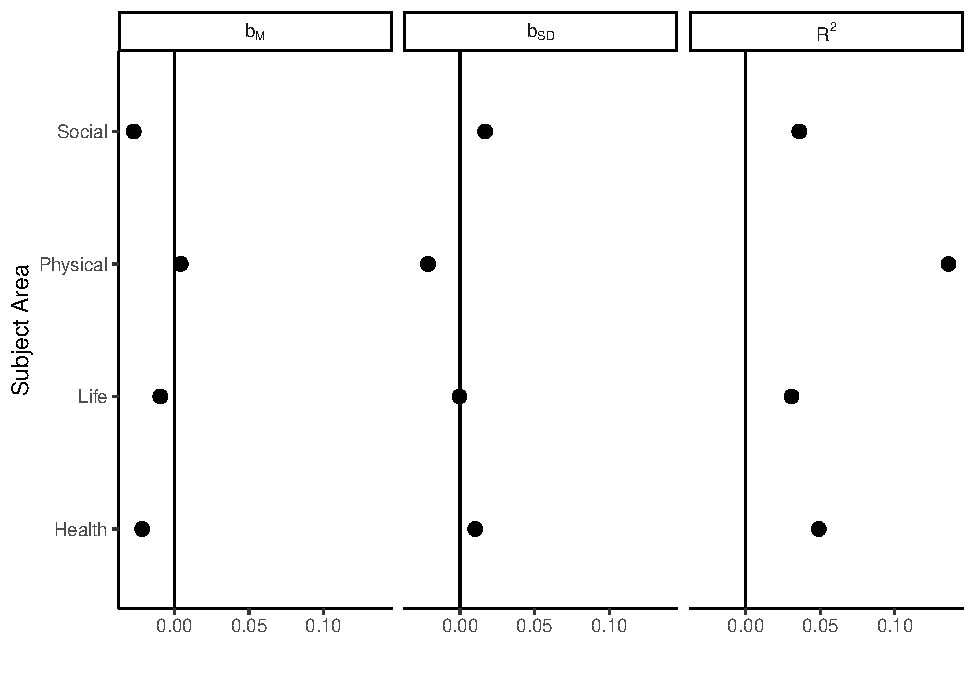
\includegraphics{manuscript_scopus_files/figure-latex/fig-pub-results-1.pdf}
\caption{\label{fig:fig-pub-results}Coefficient values for the publication totals, variance in publication totals, and the effect size for each model predicting year of publication.}
\end{figure}

\textbf{\emph{Geopolitical Regions}}.

\begin{itemize}
\tightlist
\item
  We will present visualizations of the country information listed for
  authors, and we will discuss the areas of world in which authors
  generally come from, as well as the lowest representation of
  authors.
\end{itemize}

\begin{figure}
\centering
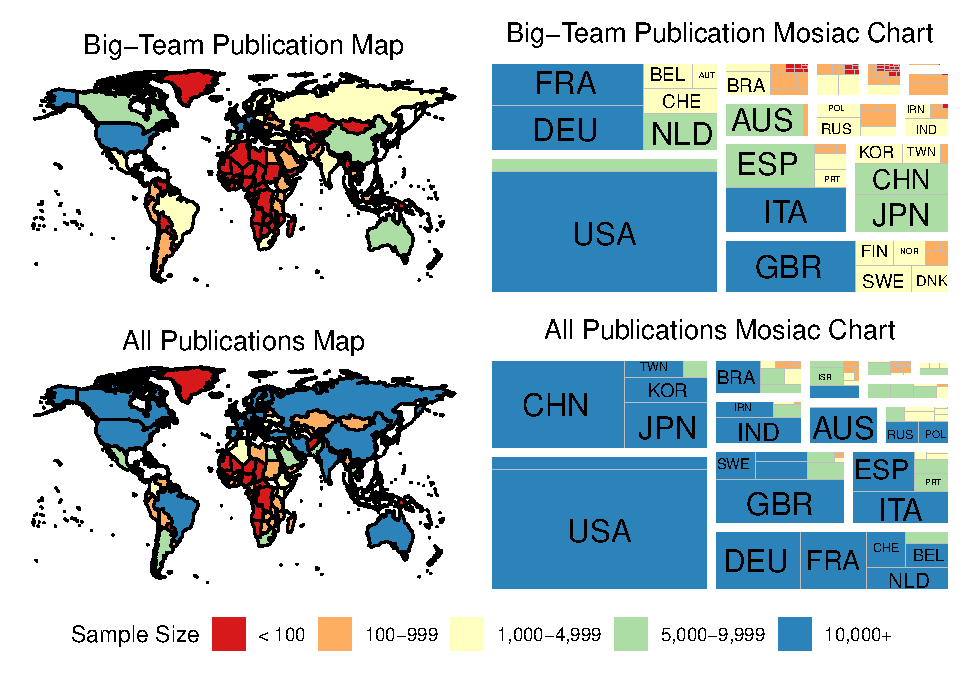
\includegraphics{manuscript_scopus_files/figure-latex/fig-map-both-1.pdf}
\caption{\label{fig:fig-map-both}Geopolitical regions represented in big-team science publications versus all publications.}
\end{figure}

\begin{itemize}
\tightlist
\item
  To understand the change in representation diversity, we will
  summarize the total number of geopolitical regions for each paper.
  Using a linear model, we will examine if the number of regions
  present is predicted by the year of publication. Increasing
  diversity would be represented by a positive slope, while decreasing
  diversity would be represented by a negative slope.
\end{itemize}

\begin{figure}
\centering
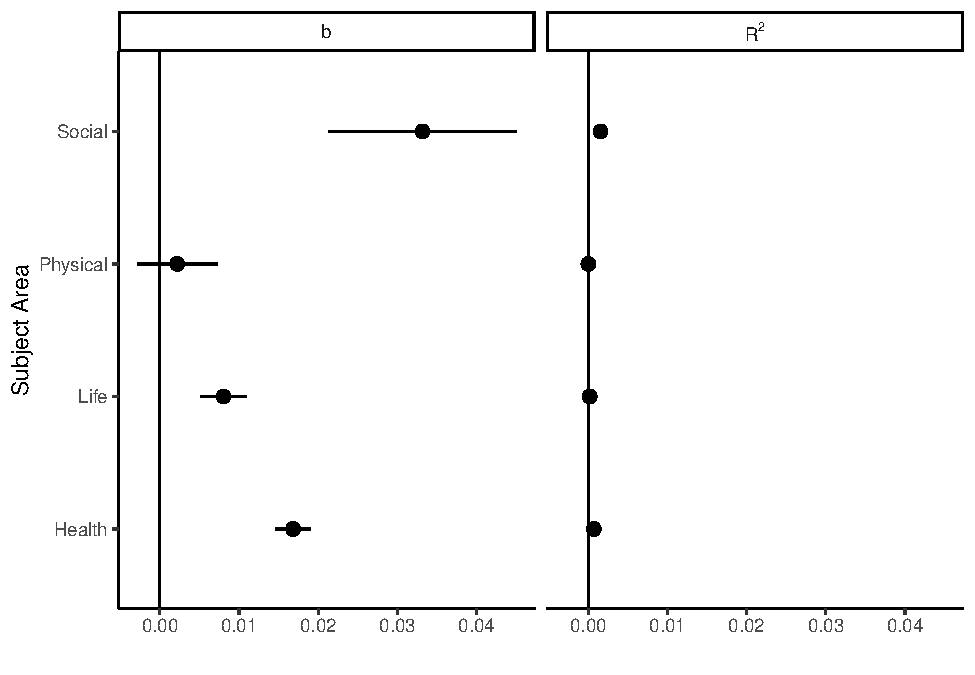
\includegraphics{manuscript_scopus_files/figure-latex/fig-diversity-1.pdf}
\caption{\label{fig:fig-diversity}Number of geopolitical regions represented in big-team science publiactions predicting time and the overall model effect size.}
\end{figure}

\begin{itemize}
\tightlist
\item
  Last, we will examine the differences in representation for
  corresponding author sets versus all other authors. For papers with
  10 to 49 authors, we will use the three first authors and the last
  author to compare against other authors. For 50 to 99 authors, five
  first authors plus last will be used, and for all papers with more
  than 100 authors, we will use ten first authors and the last author.
  We will calculate the frequencies of each of the UN Sub-Regions for
  first authors versus other authors, converting these values to
  proportions. Given the expected small sample sizes of these
  contingency tables, we will group together titles based on the year
  of publication (assuming at least 5 publications per year, these may
  be binned by 5-year or smaller increments to increase sample size).
  For each grouping, we will calculate the effect size of the
  differences in frequencies comparing first authors to all other
  authors. Since this data is categorical, we will use Cramer's \emph{V} to
  represent the effect size. If the effect size includes zero in its
  confidence interval, this result will imply that first and all other
  authors represent the same pattern of UN Sub-Region diversity. Any
  confidence interval that does include zero represents a difference
  in diversity.
\end{itemize}

\begin{figure}
\centering
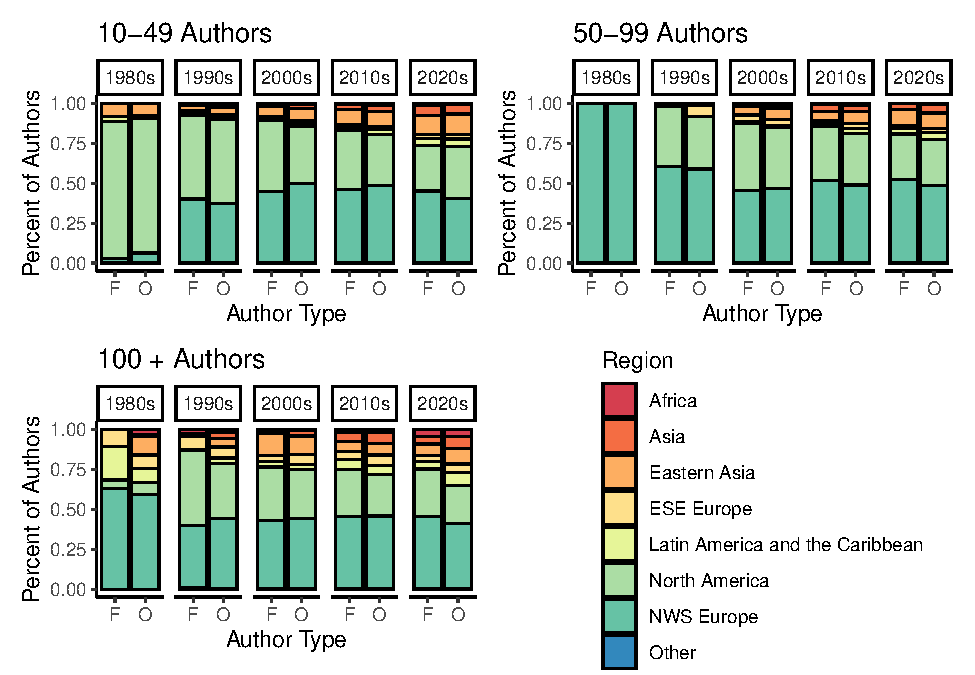
\includegraphics{manuscript_scopus_files/figure-latex/author-gpe-figure-1.pdf}
\caption{\label{fig:author-gpe-figure}A comparison of author affiliation geopolitical region across decades. F stands for first authors and O stands for other authors.}
\end{figure}

\begin{figure}
\centering
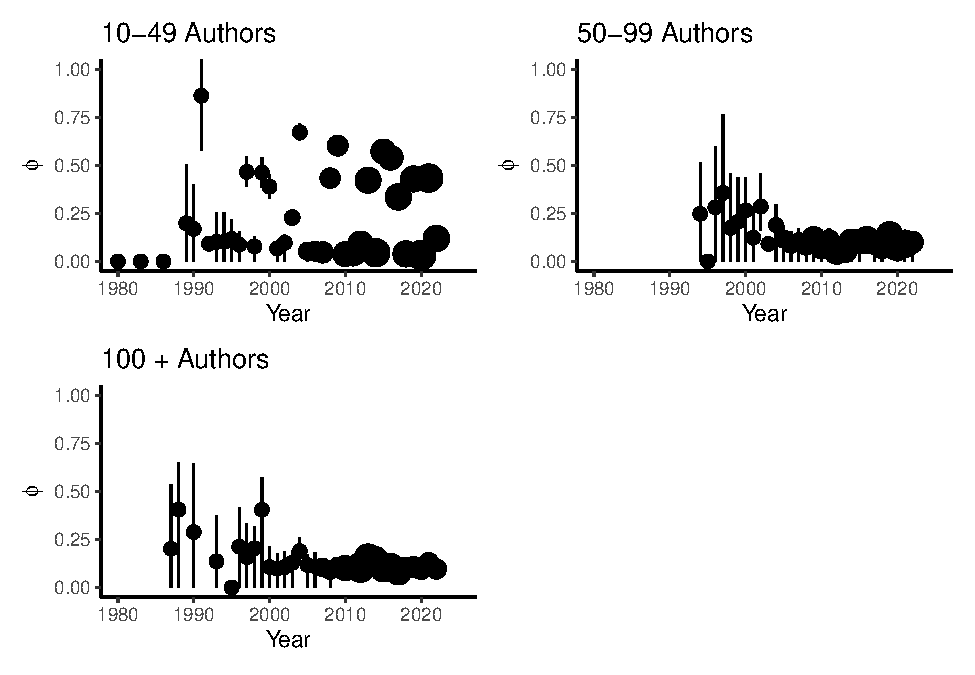
\includegraphics{manuscript_scopus_files/figure-latex/effect-gpe-figure-1.pdf}
\caption{\label{fig:effect-gpe-figure}Effect size of the differences in representation for UN Regions for author affiliations in big-team science papers by year.}
\end{figure}

\newpage

\hypertarget{references}{%
\section{References}\label{references}}

\begingroup
\setlength{\parindent}{-0.5in}
\setlength{\leftskip}{0.5in}

\hypertarget{refs}{}
\begin{CSLReferences}{1}{0}
\leavevmode\vadjust pre{\hypertarget{ref-aphilos2021}{}}%
A philosophical case for big physics. (2021). \emph{Nature Physics}, \emph{17}(6), 661--661. \url{https://doi.org/10.1038/s41567-021-01278-0}

\leavevmode\vadjust pre{\hypertarget{ref-allen2019}{}}%
Allen, L., O'Connell, A., \& Kiermer, V. (2019). How can we ensure visibility and diversity in research contributions? How the Contributor Role Taxonomy (CRediT) is helping the shift from authorship to contributorship. \emph{Learned Publishing}, \emph{32}(1), 71--74. \url{https://doi.org/10.1002/leap.1210}

\leavevmode\vadjust pre{\hypertarget{ref-auspurg2021has}{}}%
Auspurg, K., \& Brüderl, J. (2021). Has the credibility of the social sciences been credibly destroyed? Reanalyzing the {``}many analysts, one data set{''} project. \emph{Socius : Sociological Research for a Dynamic World}, \emph{7}, 23780231211024420.

\leavevmode\vadjust pre{\hypertarget{ref-bago2022}{}}%
Bago, B., Kovacs, M., Protzko, J., Nagy, T., Kekecs, Z., Palfi, B., Adamkovic, M., Adamus, S., Albalooshi, S., Albayrak-Aydemir, N., Alfian, I. N., Alper, S., Alvarez-Solas, S., Alves, S. G., Amaya, S., Andresen, P. K., Anjum, G., Ansari, D., Arriaga, P., \ldots{} Aczel, B. (2022). Situational factors shape moral judgements in the trolley dilemma in Eastern, Southern and Western countries in a culturally diverse sample. \emph{Nature Human Behaviour}, 1--13. \url{https://doi.org/10.1038/s41562-022-01319-5}

\leavevmode\vadjust pre{\hypertarget{ref-buttrick2020}{}}%
Buttrick, N. R., Aczel, B., Aeschbach, L. F., Bakos, B. E., Brühlmann, F., Claypool, H. M., Hüffmeier, J., Kovacs, M., Schuepfer, K., Szecsi, P., Szuts, A., Szöke, O., Thomae, M., Torka, A.-K., Walker, R. J., \& Wood, M. J. (2020). Many Labs 5: Registered Replication of Vohs and Schooler (2008), Experiment 1. \emph{Advances in Methods and Practices in Psychological Science}, \emph{3}(3), 429--438. \url{https://doi.org/10.1177/2515245920917931}

\leavevmode\vadjust pre{\hypertarget{ref-castelnovo2018}{}}%
Castelnovo, P., Florio, M., Forte, S., Rossi, L., \& Sirtori, E. (2018). The economic impact of technological procurement for large-scale research infrastructures: Evidence from the Large Hadron Collider at CERN. \emph{Research Policy}, \emph{47}(9), 1853--1867. \url{https://doi.org/10.1016/j.respol.2018.06.018}

\leavevmode\vadjust pre{\hypertarget{ref-coles2022}{}}%
Coles, N. A., Hamlin, J. K., Sullivan, L. L., Parker, T. H., \& Altschul, D. (2022). Build up big-team science. \emph{Nature}, \emph{601}(7894), 505--507. \url{https://doi.org/10.1038/d41586-022-00150-2}

\leavevmode\vadjust pre{\hypertarget{ref-collins2003}{}}%
Collins, F. S., Morgan, M., \& Patrinos, A. (2003). The human genome project: Lessons from large-scale biology. \emph{Science}, \emph{300}(5617), 286--290. \url{https://doi.org/10.1126/science.1084564}

\leavevmode\vadjust pre{\hypertarget{ref-dorison2022}{}}%
Dorison, C., Lerner, J., Heller, B., Rothman, A., Kawachi, I., Wang, K., Rees, V., Gill, B., Gibbs, N., Ebersole, C., Vally, Z., Tajchman, Z., Zsido, A., Zrimsek, M., Chen, Z., Ziano, I., Gialitaki, Z., Ceary, C., Jang, Y., \ldots{} Coles, N. (2022). A global test of message framing on behavioural intentions, policy support, information seeking, and experienced anxiety during the COVID-19 pandemic. \emph{Affective Science}. \url{https://doi.org/10.31234/osf.io/sevkf}

\leavevmode\vadjust pre{\hypertarget{ref-ebersole2016}{}}%
Ebersole, C. R., Atherton, O. E., Belanger, A. L., Skulborstad, H. M., Allen, J. M., Banks, J. B., Baranski, E., Bernstein, M. J., Bonfiglio, D. B. V., Boucher, L., Brown, E. R., Budiman, N. I., Cairo, A. H., Capaldi, C. A., Chartier, C. R., Chung, J. M., Cicero, D. C., Coleman, J. A., Conway, J. G., \ldots{} Nosek, B. A. (2016). Many Labs 3: Evaluating participant pool quality across the academic semester via replication. \emph{Journal of Experimental Social Psychology}, \emph{67}, 68--82. \url{https://doi.org/10.1016/j.jesp.2015.10.012}

\leavevmode\vadjust pre{\hypertarget{ref-ebersole2020}{}}%
Ebersole, C. R., Mathur, M. B., Baranski, E., Bart-Plange, D.-J., Buttrick, N. R., Chartier, C. R., Corker, K. S., Corley, M., Hartshorne, J. K., IJzerman, H., Lazarević, L. B., Rabagliati, H., Ropovik, I., Aczel, B., Aeschbach, L. F., Andrighetto, L., Arnal, J. D., Arrow, H., Babincak, P., \ldots{} Nosek, B. A. (2020). Many Labs 5: Testing Pre-Data-Collection Peer Review as an Intervention to Increase Replicability. \emph{Advances in Methods and Practices in Psychological Science}, \emph{3}(3), 309--331. \url{https://doi.org/10.1177/2515245920958687}

\leavevmode\vadjust pre{\hypertarget{ref-10.7554ux2feLife.71601}{}}%
Errington, T. M., Mathur, M., Soderberg, C. K., Denis, A., Perfito, N., Iorns, E., \& Nosek, B. A. (2021). Investigating the replicability of preclinical cancer biology. \emph{eLife}, \emph{10}, e71601. \url{https://doi.org/10.7554/eLife.71601}

\leavevmode\vadjust pre{\hypertarget{ref-forscher2020}{}}%
Forscher, P. S., Wagenmakers, E.-J., Coles, N. A., Silan, M. A. A., Dutra, N. B., Basnight-Brown, D., \& IJzerman, H. (2020). \emph{The benefits, barriers, and risks of big team science}. \url{https://doi.org/10.31234/osf.io/2mdxh}

\leavevmode\vadjust pre{\hypertarget{ref-franco2014}{}}%
Franco, A., Malhotra, N., \& Simonovits, G. (2014). Publication bias in the social sciences: Unlocking the file drawer. \emph{Science}, \emph{345}(6203), 1502--1505. \url{https://doi.org/10.1126/science.1255484}

\leavevmode\vadjust pre{\hypertarget{ref-grahe2014}{}}%
Grahe, J. E. (2014). Announcing open science badges and reaching for the sky. \emph{The Journal of Social Psychology}, \emph{154}(1), 1--3. \url{https://doi.org/10.1080/00224545.2014.853582}

\leavevmode\vadjust pre{\hypertarget{ref-henrich2010}{}}%
Henrich, J., Heine, S. J., \& Norenzayan, A. (2010). The weirdest people in the world? \emph{Behavioral and Brain Sciences}, \emph{33}(2-3), 61--83. \url{https://doi.org/10.1017/S0140525X0999152X}

\leavevmode\vadjust pre{\hypertarget{ref-hubbard1997}{}}%
Hubbard, R., \& Armstrong, J. S. (1997). Publication Bias against Null Results. \emph{Psychological Reports}, \emph{80}(1), 337--338. \url{https://doi.org/10.2466/pr0.1997.80.1.337}

\leavevmode\vadjust pre{\hypertarget{ref-ioannidis2015}{}}%
Ioannidis, J. P. A. (2015). Failure to replicate: Sound the alarm. \emph{Cerebrum: The Dana Forum on Brain Science}, \emph{2015}. \url{https://www.ncbi.nlm.nih.gov/pmc/articles/PMC4938249/}

\leavevmode\vadjust pre{\hypertarget{ref-isager2021}{}}%
Isager, P. M., Aert, R. C. M. van, Bahník, Š., Brandt, M. J., DeSoto, K. A., Giner-Sorolla, R., Krueger, J. I., Perugini, M., Ropovik, I., van 't Veer, A. E., Vranka, M., \& Lakens, D. (2021a). Deciding what to replicate: A decision model for replication study selection under resource and knowledge constraints. \emph{Psychological Methods}. \url{https://doi.org/10.1037/met0000438}

\leavevmode\vadjust pre{\hypertarget{ref-isager2021a}{}}%
Isager, P. M., Aert, R. C. M. van, Bahník, Š., Brandt, M. J., DeSoto, K. A., Giner-Sorolla, R., Krueger, J. I., Perugini, M., Ropovik, I., van 't Veer, A. E., Vranka, M., \& Lakens, D. (2021b). Deciding what to replicate: A decision model for replication study selection under resource and knowledge constraints. \emph{Psychological Methods}. \url{https://doi.org/10.1037/met0000438}

\leavevmode\vadjust pre{\hypertarget{ref-john2012}{}}%
John, L. K., Loewenstein, G., \& Prelec, D. (2012). Measuring the Prevalence of Questionable Research Practices With Incentives for Truth Telling. \emph{Psychological Science}, \emph{23}(5), 524--532. \url{https://doi.org/10.1177/0956797611430953}

\leavevmode\vadjust pre{\hypertarget{ref-jones2021}{}}%
Jones, B. C., DeBruine, L. M., Flake, J. K., Liuzza, M. T., Antfolk, J., Arinze, N. C., Ndukaihe, I. L. G., Bloxsom, N. G., Lewis, S. C., Foroni, F., Willis, M. L., Cubillas, C. P., Vadillo, M. A., Turiegano, E., Gilead, M., Simchon, A., Saribay, S. A., Owsley, N. C., Jang, C., \ldots{} Coles, N. A. (2021). To which world regions does the valence{\textendash}dominance model of social perception apply? \emph{Nature Human Behaviour}, \emph{5}(1), 159--169. \url{https://doi.org/10.1038/s41562-020-01007-2}

\leavevmode\vadjust pre{\hypertarget{ref-kidwell2016}{}}%
Kidwell, M. C., Lazarević, L. B., Baranski, E., Hardwicke, T. E., Piechowski, S., Falkenberg, L.-S., Kennett, C., Slowik, A., Sonnleitner, C., Hess-Holden, C., Errington, T. M., Fiedler, S., \& Nosek, B. A. (2016). Badges to Acknowledge Open Practices: A Simple, Low-Cost, Effective Method for Increasing Transparency. \emph{PLOS Biology}, \emph{14}(5), e1002456. \url{https://doi.org/10.1371/journal.pbio.1002456}

\leavevmode\vadjust pre{\hypertarget{ref-klein2022}{}}%
Klein, R. A., Cook, C. L., Ebersole, C. R., Vitiello, C., Nosek, B. A., Hilgard, J., Ahn, P. H., Brady, A. J., Chartier, C. R., Christopherson, C. D., Clay, S., Collisson, B., Crawford, J. T., Cromar, R., Gardiner, G., Gosnell, C. L., Grahe, J., Hall, C., Howard, I., \ldots{} Ratliff, K. A. (2022). Many Labs 4: Failure to Replicate Mortality Salience Effect With and Without Original Author Involvement. \emph{Collabra: Psychology}, \emph{8}(1), 35271. \url{https://doi.org/10.1525/collabra.35271}

\leavevmode\vadjust pre{\hypertarget{ref-klein2018}{}}%
Klein, R. A., Vianello, M., Hasselman, F., Adams, B. G., Adams, R. B., Alper, S., Aveyard, M., Axt, J. R., Babalola, M. T., Bahník, Š., Batra, R., Berkics, M., Bernstein, M. J., Berry, D. R., Bialobrzeska, O., Binan, E. D., Bocian, K., Brandt, M. J., Busching, R., \ldots{} Nosek, B. A. (2018). Many Labs 2: Investigating Variation in Replicability Across Samples and Settings. \emph{Advances in Methods and Practices in Psychological Science}, \emph{1}(4), 443--490. \url{https://doi.org/10.1177/2515245918810225}

\leavevmode\vadjust pre{\hypertarget{ref-lebel2018}{}}%
LeBel, E. P., McCarthy, R. J., Earp, B. D., Elson, M., \& Vanpaemel, W. (2018). A Unified Framework to Quantify the Credibility of Scientific Findings. \emph{Advances in Methods and Practices in Psychological Science}, \emph{1}(3), 389--402. \url{https://doi.org/10.1177/2515245918787489}

\leavevmode\vadjust pre{\hypertarget{ref-legate2022}{}}%
Legate, N., Nguyen, T., Weinstein, N., Moller, A., Legault, L., Maniaci, M. R., Ebersole, C. R., Adamkovic, M., Adetula, D. G. A., Agesin, B. B., Ahlgren, L., Akkas, H., Almeida, I., Anjum, G., Antoniadi, M., Arinze, A. I., Arvanitis, A., Rana, K., Badalyan, V., \ldots{} Primbs, M. (2022). A global experiment on motivating social distancing during the COVID-19 pandemic. \emph{Proceedings of the National Academy of Sciences}. \url{https://doi.org/10.31234/osf.io/n3dyf}

\leavevmode\vadjust pre{\hypertarget{ref-maizey2019}{}}%
Maizey, L., \& Tzavella, L. (2019). Barriers and solutions for early career researchers in tackling the reproducibility crisis in cognitive neuroscience. \emph{Cortex}, \emph{113}, 357--359. \url{https://doi.org/10.1016/j.cortex.2018.12.015}

\leavevmode\vadjust pre{\hypertarget{ref-mathur2020}{}}%
Mathur, M. B., Bart-Plange, D.-J., Aczel, B., Bernstein, M. H., Ciunci, A. M., Ebersole, C. R., Falcão, F., Ashbaugh, K., Hilliard, R. A., Jern, A., Kellier, D. J., Kessinger, G., Kolb, V. S., Kovacs, M., Lage, C. A., Langford, E. V., Lins, S., Manfredi, D., Meyet, V., \ldots{} Frank, M. C. (2020). Many Labs 5: Registered Multisite Replication of the Tempting-Fate Effects in Risen and Gilovich (2008). \emph{Advances in Methods and Practices in Psychological Science}, \emph{3}(3), 394--404. \url{https://doi.org/10.1177/2515245918785165}

\leavevmode\vadjust pre{\hypertarget{ref-maxwell2015}{}}%
Maxwell, S. E., Lau, M. Y., \& Howard, G. S. (2015). Is psychology suffering from a replication crisis?: What does 'failure to replicate' really mean? \emph{American Psychologist}, \emph{70}(6), 487--498. \url{https://doi.org/10.1037/a0039400}

\leavevmode\vadjust pre{\hypertarget{ref-mayo-wilson2021}{}}%
Mayo-Wilson, E., Grant, S., Supplee, L., Kianersi, S., Amin, A., DeHaven, A., \& Mellor, D. (2021). Evaluating implementation of the transparency and openness promotion~(TOP) guidelines:~The TRUST process for rating journal policies, procedures, and practices. \emph{Research Integrity and Peer Review}, \emph{6}(1), 9. \url{https://doi.org/10.1186/s41073-021-00112-8}

\leavevmode\vadjust pre{\hypertarget{ref-moshontz2018}{}}%
Moshontz, H., Campbell, L., Ebersole, C. R., IJzerman, H., Urry, H. L., Forscher, P. S., Grahe, J. E., McCarthy, R. J., Musser, E. D., Antfolk, J., Castille, C. M., Evans, T. R., Fiedler, S., Flake, J. K., Forero, D. A., Janssen, S. M. J., Keene, J. R., Protzko, J., Aczel, B., \ldots{} Chartier, C. R. (2018). The Psychological Science Accelerator: Advancing Psychology Through a Distributed Collaborative Network. \emph{Advances in Methods and Practices in Psychological Science}, \emph{1}(4), 501--515. \url{https://doi.org/10.1177/2515245918797607}

\leavevmode\vadjust pre{\hypertarget{ref-nelson2018}{}}%
Nelson, L. D., Simmons, J., \& Simonsohn, U. (2018). Psychology's renaissance. \emph{Annual Review of Psychology}, \emph{69}(1), 511--534. \url{https://doi.org/10.1146/annurev-psych-122216-011836}

\leavevmode\vadjust pre{\hypertarget{ref-newson2021}{}}%
Newson, M., Buhrmester, M., Xygalatas, D., \& Whitehouse, H. (2021). Go WILD, not WEIRD. \emph{Journal for the Cognitive Science of Religion}, \emph{6}(1-2). \url{https://doi.org/10.1558/jcsr.38413}

\leavevmode\vadjust pre{\hypertarget{ref-nosek2015}{}}%
Nosek, B. A., Alter, G., Banks, G. C., Borsboom, D., Bowman, S. D., Breckler, S. J., Buck, S., Chambers, C. D., Chin, G., Christensen, G., Contestabile, M., Dafoe, A., Eich, E., Freese, J., Glennerster, R., Goroff, D., Green, D. P., Hesse, B., Humphreys, M., \ldots{} Yarkoni, T. (2015). Promoting an open research culture. \emph{Science}, \emph{348}(6242), 1422--1425. \url{https://doi.org/10.1126/science.aab2374}

\leavevmode\vadjust pre{\hypertarget{ref-nosek2014}{}}%
Nosek, B. A., \& Lakens, D. (2014a). Registered Reports: A Method to Increase the Credibility of Published Results. \emph{Social Psychology}, \emph{45}(3), 137--141. \url{https://doi.org/10.1027/1864-9335/a000192}

\leavevmode\vadjust pre{\hypertarget{ref-nosek2014method}{}}%
Nosek, B. A., \& Lakens, D. (2014b). A method to increase the credibility of published results. \emph{Social Psychology}, \emph{45}(3), 137141.

\leavevmode\vadjust pre{\hypertarget{ref-nosek2012}{}}%
Nosek, B. A., Spies, J. R., \& Motyl, M. (2012). Scientific Utopia: II. Restructuring Incentives and Practices to Promote Truth Over Publishability. \emph{Perspectives on Psychological Science}, \emph{7}(6), 615--631. \url{https://doi.org/10.1177/1745691612459058}

\leavevmode\vadjust pre{\hypertarget{ref-oed2016}{}}%
OED. (2016). \emph{Collaboration} (Vol. 3). Oxford University.

\leavevmode\vadjust pre{\hypertarget{ref-opensciencecollaboration2015}{}}%
Open Science Collaboration. (2015). Estimating the reproducibility of psychological science. \emph{Science}, \emph{349}(6251), aac4716--aac4716. \url{https://doi.org/10.1126/science.aac4716}

\leavevmode\vadjust pre{\hypertarget{ref-rad2018}{}}%
Rad, M. S., Martingano, A. J., \& Ginges, J. (2018). Toward a psychology of homo sapiens: Making psychological science more representative of the human population. \emph{Proceedings of the National Academy of Sciences}, \emph{115}(45), 11401--11405. \url{https://doi.org/10.1073/pnas.1721165115}

\leavevmode\vadjust pre{\hypertarget{ref-silberzahn2018many}{}}%
Silberzahn, R., Uhlmann, E. L., Martin, D. P., Anselmi, P., Aust, F., Awtrey, E., Bahník, Š., Bai, F., Bannard, C., Bonnier, E., \& others. (2018). Many analysts, one data set: Making transparent how variations in analytic choices affect results. \emph{Advances in Methods and Practices in Psychological Science}, \emph{1}(3), 337356.

\leavevmode\vadjust pre{\hypertarget{ref-skorb2020}{}}%
Skorb, L., Aczel, B., Bakos, B. E., Feinberg, L., Hałasa, E., Kauff, M., Kovacs, M., Krasuska, K., Kuchno, K., Manfredi, D., Montealegre, A., Pękala, E., Pieńkosz, D., Ravid, J., Rentzsch, K., Szaszi, B., Schulz-Hardt, S., Sioma, B., Szecsi, P., \ldots{} Hartshorne, J. K. (2020). Many Labs 5: Replication of van Dijk, van Kleef, Steinel, and van Beest (2008). \emph{Advances in Methods and Practices in Psychological Science}, \emph{3}(3), 418--428. \url{https://doi.org/10.1177/2515245920927643}

\leavevmode\vadjust pre{\hypertarget{ref-stewart2017}{}}%
Stewart, N., Chandler, J., \& Paolacci, G. (2017). Crowdsourcing samples in cognitive science. \emph{Trends in Cognitive Sciences}, \emph{21}(10), 736--748. \url{https://doi.org/10.1016/j.tics.2017.06.007}

\leavevmode\vadjust pre{\hypertarget{ref-stewart2020}{}}%
Stewart, S., Rinke, E. M., McGarrigle, R., Lynott, D., Lunny, C., Lautarescu, A., Galizzi, M. M., Farran, E. K., \& Crook, Z. (2020). \emph{Pre-registration and registered reports: A primer from UKRN}. \url{https://doi.org/10.31219/osf.io/8v2n7}

\leavevmode\vadjust pre{\hypertarget{ref-vanbavel2022}{}}%
Van Bavel, J. J., Cichocka, A., Capraro, V., Sjåstad, H., Nezlek, J. B., Pavlović, T., Alfano, M., Gelfand, M. J., Azevedo, F., Birtel, M. D., Cislak, A., Lockwood, P. L., Ross, R. M., Abts, K., Agadullina, E., Aruta, J. J. B., Besharati, S. N., Bor, A., Choma, B. L., \ldots{} Boggio, P. S. (2022). National identity predicts public health support during a global pandemic. \emph{Nature Communications}, \emph{13}(1), 517. \url{https://doi.org/10.1038/s41467-021-27668-9}

\leavevmode\vadjust pre{\hypertarget{ref-vazire2022}{}}%
Vazire, S., Schiavone, S. R., \& Bottesini, J. G. (2022). Credibility Beyond Replicability: Improving the Four Validities in Psychological Science. \emph{Current Directions in Psychological Science}, \emph{31}(2), 162--168. \url{https://doi.org/10.1177/09637214211067779}

\leavevmode\vadjust pre{\hypertarget{ref-wang2021}{}}%
Wang, K., Goldenberg, A., Dorison, C. A., Miller, J. K., Uusberg, A., Lerner, J. S., Gross, J. J., Agesin, B. B., Bernardo, M., Campos, O., Eudave, L., Grzech, K., Ozery, D. H., Jackson, E. A., Garcia, E. O. L., Drexler, S. M., Jurković, A. P., Rana, K., Wilson, J. P., \ldots{} Moshontz, H. (2021). A multi-country test of brief reappraisal interventions on emotions during the COVID-19 pandemic. \emph{Nature Human Behaviour}, \emph{5}(8), 1089--1110. \url{https://doi.org/10.1038/s41562-021-01173-x}

\leavevmode\vadjust pre{\hypertarget{ref-zwaan2018}{}}%
Zwaan, R. A., Etz, A., Lucas, R. E., \& Donnellan, M. B. (2018). Making replication mainstream. \emph{Behavioral and Brain Sciences}, \emph{41}, e120. \url{https://doi.org/10.1017/S0140525X17001972}

\end{CSLReferences}

\endgroup


\end{document}
